%
% anwendungen.tex -- Anwendungen des Reed-Solomon-Codes
%
% (c) 2021 Michael Steiner, Hochschule Rapperswil
%
\section{Anwendungen des Reed-Solomon-Codes
	\label{reedsolomon:section:anwendung}}
\rhead{Anwendungen}
\textcolor{red}{Platzierung der Bilder? Quellenangabe der Bilder?}

In den vorherigen Abschnitten haben wir betrachtet, wie Reed-Solomon-Codes in der Theorie Funktionieren. 
In diesem Abschnitt werden wir einige Anwendungen vorstellen, bei denen ein Reed-Solomon-Code zum Einsatz kommt.
Obwohl alle diese Codes nach dem gleichen Prinzip arbeiten gibt es starke Unterschiede in deren Funktionsweise. 
Dies kommt vor allem daher, da die Codes nur Ressourcen zur Verfügung haben, die von der Hardware bereitstellt wird,  auf denen die Codes implementiert wurden.
Diese Codes bedienen sich daher verschiedener Tricks und Optimierungen um möglichst effizient zu arbeiten.
%
%Dies kommt vor allem daher, da diese Codes an ihre Hardware gebunden sind, auf denen sie implementiert worden sind.
%Deshalb wurden diese Codes stark optimiert damit sie möglichst Effizient arbeiten können. 
%
%Um diese Hardware möglichst effizient zu nutzen wurden gewisse mathematische tricks angewendet um den Code möglichst effizient zu nutzen. 
%
% um mit maximaler Effizienz zu arbeiten. 
%Es überrascht daher nicht, dass vor allem ältere Codes im binären Körper $\mathbb{F}_{2}$ arbeiten.
%
% um den Code mit maximaler Effizienz zu nutzen. 
%
%Alle diese Anwendungen verfügen über eigene spezifizierten Eigenschaften.
%
%, wobei bei allen dieser Anwendungen jeweils eine unterschiedliche Version des Codes implementiert wurden.
%
%Dies kommt vor allem daher, da diese Codes immer an ihre dementsprechende Hardware gebunden sind, auf denen sie implementiert wurden um den Code mit maximaler Effizienz zu nutzen. 
%
% eigene Version des Codes implementiert haben. 
%
%Bei einer Technischen Umsetzung eines solchen Codes werden wir auf eine reihe neuer Probleme stossen wie Ressourceneffizienz, Laufzeitoptimierung, usw.
%
%Hinzu kommt, dass für verschiedene Anwendungen verschiedene Versionen des Reed-Solomon-Codes zur Anwendung kommen.
%
%Nachfolgend werden wir ein paar dieser Anwendungen Vorstellen, da sich herausstellt, dass Reed-Solomon-Code sehr 
%
%Als letzte Frage stellt sich jetzt nur noch, wo diese Codes eingesetzt werden. 
%
%Bisher haben wir 
%
%In den letzten abschnitten haben wir uns ausführlich die Funktionsweise des Reed-Solomon-Codes angeschaut. In diesem Abschnitt möchten wir dem Leser ein paar bekannte beispiele vorstellen, in denen Reed-Solomon-Codes zum einsatz kommen. Es sei jedoch angemerkt, dass diese Anwendungen in der Umsetzung oft ein wenig anderst funktionieren als hier vorgestellt. Dies wurde vor allem wegen technischen optimierungen realisiert. (technische tricks und finessen), von der logik jedoch sehr stark an unserem Beispiel orientieren

\subsection{Raumfahrt}
Obwohl Reed-Solomon-Codes bereits in den 1960er entwickelt wurden fanden sie erstmals Anwendung in der Voyager Raumsonde der NASA. Die Daten der zwei im Jahre 1977 gestarteten Sonden werden mit einem RS(255,233)-Code \textcolor{red}{benötigt das weitere erklärungen, wie z.b. 255: grösse nachrichtenblock, 233: anzahl der nutzbaren daten ?} zusammen mit einem konventionellen Faltungscode übertragen. 

%
% Die zwei im Jahre 1977 gestarteten Sonden senden Daten mit der Hilfe eines RS(255,233)-Code für die digitalen Bilder sowie einem konventionellen Faltungscode.
%
%
%mit der Erde mit einem RS(255,233)-Code für die digitalen Bilder sowie einem konventionellen Faltungscode. 

\begin{figure}
	\centering
	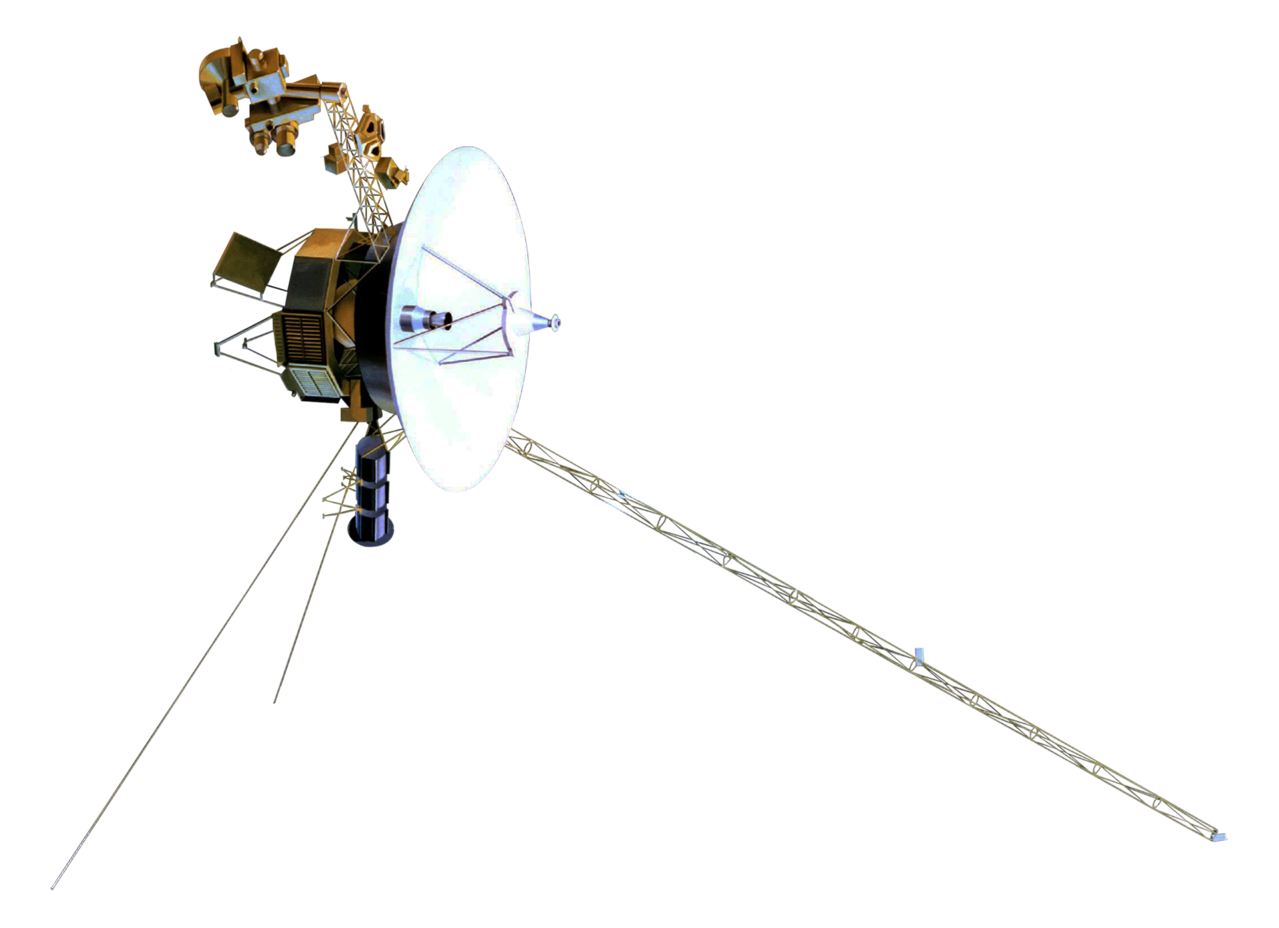
\includegraphics[width=0.5\textwidth]{papers/reedsolomon/images/Voyager_Sonde}
	\caption{Voyager Raumsonde}
	\label{fig:voyager}
\end{figure}

\subsection{CD/DVD}
Compact discs verwenden sogar zwei ineinander verschachtelte Reed-Solomon-Codes, einen (32,28)-Code und einen (28,24)-Code.
Beide Codes sind in der Lage, Fehler aus dem jeweils anderen gelesenen Block zu korrigieren. Dieses spezielle zusammenspielen dieser beiden Codes werden auch Cross-interleaved Reed-Solomon-Codes (CIRC) genannt.
Diese Vorgehensweise erzielt eine hohe Robustheit gegenüber Produktionsfehler oder Verschmutzung auf der Disc. Bei CD's sind diese in der Lage bis zu 4000 fehlerhafte Bits am Stück (ca. $2.5mm$) zu erkennen und zu korrigieren. 

Die Digital Video Disc funktioniert nach dem selben Konzept mit grösseren Codeblöcken. Die DVD verwendet einen (208,192)-Code und einen (182,172)-Code.

%Beide lesen 
% wobei beide Codes auch Fehler aus dem jeweiligen anderen Block korrigieren

\begin{figure}
	\centering
	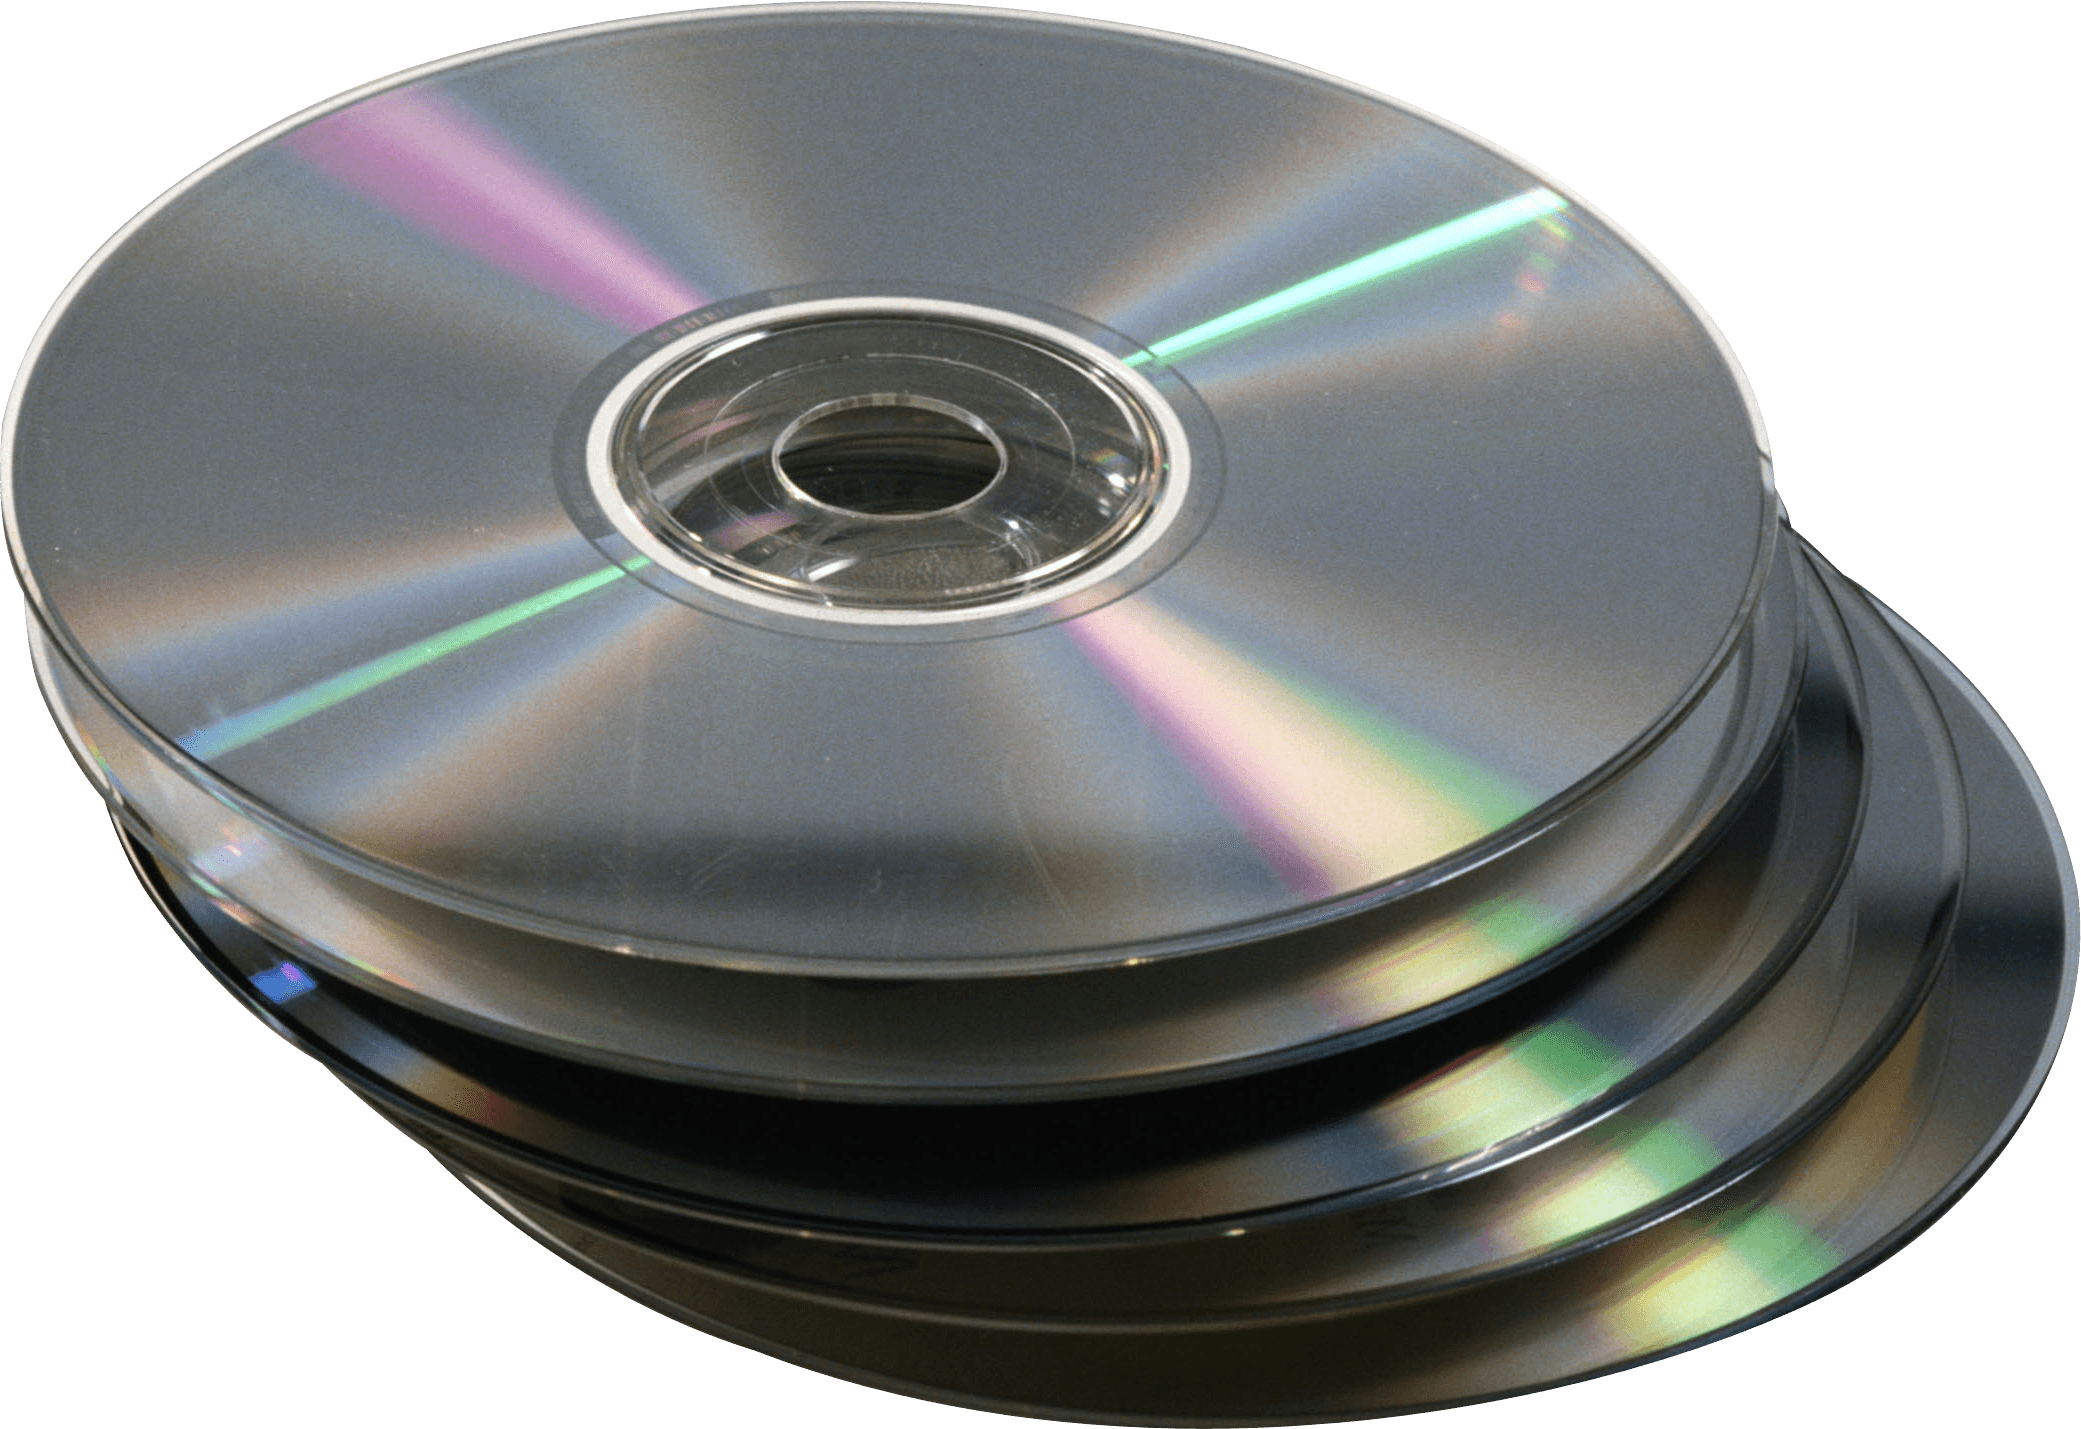
\includegraphics[width=0.5\textwidth]{papers/reedsolomon/images/Compact_Disc}
	\caption{Compact Disc}
	\label{fig:cd}
\end{figure}

\subsection{QR-Codes}
Quick Response Codes funktionieren nach einem sehr ähnlichen Prinzip wie in unserem Beispiel, nur dass QR-Codes in einem $\mathbb{F}_{256}$ Körper arbeiten. Je nach grösse der Codierung ist der QR-Code im Endeffekt robuster gegen Beschädigungen. Bei Low Level Codes können 7\% der Daten Wiederhergestellt werden, beim High Level Code sind das sogar 30\%.

\begin{figure}
	\centering
	\subfigure[]{
	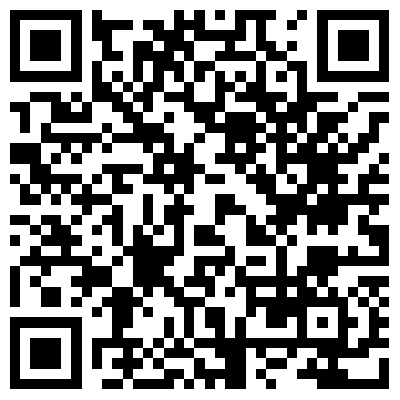
\includegraphics[width=0.4\textwidth]{papers/reedsolomon/images/qrcode_h}
	}
	\subfigure[]{
	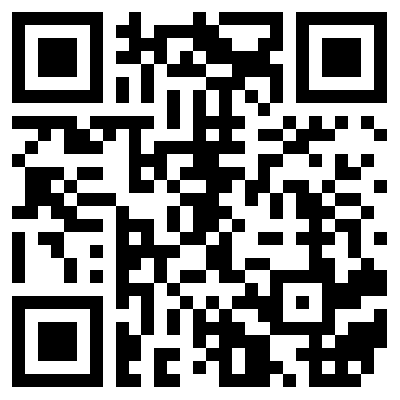
\includegraphics[width=0.4\textwidth]{papers/reedsolomon/images/qrcode_l}
	}
	\caption{(a) High Level Code, (b) Low Level Code}
	\label{fig:qr}
\end{figure}
